\documentclass[tikz,border=12pt]{standalone}
\usepackage{amsmath,amssymb}
\usetikzlibrary{calc,arrows.meta,patterns}

\begin{document}
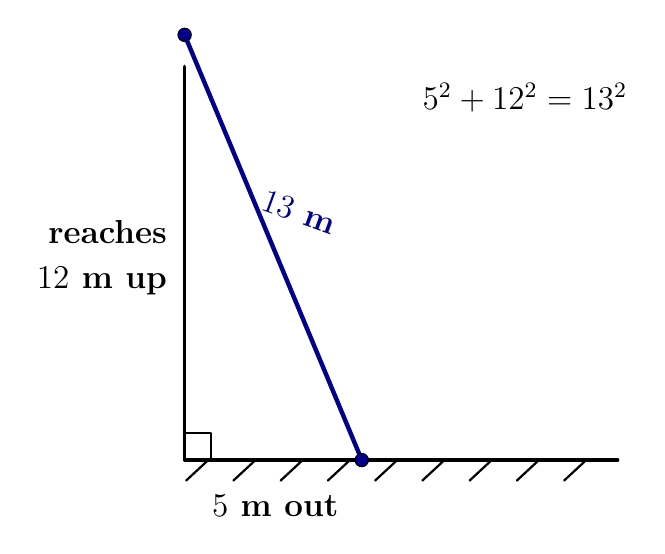
\begin{tikzpicture}[>=latex, line cap=round, line join=round]

  % Wall and ground
  \draw[very thick] (0,0) -- (0,5.0);
  \draw[very thick] (0,0) -- (5.5,0);
  % cobbles on the ground
  \foreach \x in {0.3,0.9,...,5.4}{\draw[thick] (\x,0) -- (\x-0.28,-0.26);}

  % Ladder (scaled 0.45): base foot 5 m out -> (2.25,0); reach 12 m -> (0,5.4)
  \coordinate (T) at (0,5.4);
  \coordinate (F) at (2.25,0);
  \draw[ultra thick, blue!55!black] (T) -- (F);
  \draw[fill=blue!55!black] (T) circle (2.4pt);
  \draw[fill=blue!55!black] (F) circle (2.4pt);

  % right angle at the wall base
  \draw[thick] (0,0.34) -- (0.34,0.34) -- (0.34,0);

  % labels
  \node[blue!55!black, font=\large\bfseries, rotate=-20] at (1.45,3.15) {$13$ m};
  \node[font=\large\bfseries, below] at (1.15,-0.32) {$5$ m out};
  \node[font=\large\bfseries, left] at (-0.1,2.9) {reaches};
  \node[font=\large\bfseries, left] at (-0.1,2.28) {$12$ m up};

  \node[font=\large, anchor=west] at (2.9,4.6)
    {$5^2 + 12^2 = 13^2$};

\end{tikzpicture}
\end{document}
